\documentclass[a4paper,11pt]{article}
\usepackage[T1]{fontenc}
\usepackage[utf8]{inputenc}
\usepackage{lmodern,amsmath,amssymb,amsthm,booktabs,array,microtype}
\usepackage[margin=.9in]{geometry}
\usepackage[hidelinks]{hyperref}
\hypersetup{pdftitle={An almost-entropic Ingleton score below -0.09738},
pdfauthor={Soren Riis (creator and coordinator)},
pdfsubject={Preprint and Lean proof; DOI 10.5281/zenodo.23662511},
pdfkeywords={entropy region, Ingleton inequality, almost-entropic cone, privacy amplification, Lean}}
\usepackage{enumitem,tikz}
\setlist{nosep}
\newtheorem{theorem}{Theorem}
\newtheorem{lemma}[theorem]{Lemma}
\newtheorem{proposition}[theorem]{Proposition}
\newtheorem{corollary}[theorem]{Corollary}
\newcommand{\F}{\mathbb F_2}
\newcommand{\AEcone}{\overline{\Gamma_4^{*}}}
\newcommand{\E}{\mathbb E}
\newcommand{\TV}{\operatorname{TV}}
\newcommand{\rank}{\operatorname{rank}}
\newcommand{\Ing}{\operatorname{J}}
\newcommand{\hb}{h_2}
\DeclareMathOperator{\supp}{supp}
\title{An almost-entropic Ingleton score below $-0.09738$\\[3pt]
\large Conditional hashing of a binary parity structure}
\author{S\o ren Riis\thanks{Creator and coordinator. Research direction, contributions and AI assistance are described at the end of the paper.}}
\date{}
\renewcommand{\thesection}{\Roman{section}}
\renewcommand{\thesubsection}{\Alph{subsection}}
\begin{document}
\setlength{\abovedisplayskip}{8pt}
\setlength{\belowdisplayskip}{8pt}
\maketitle
\vspace{-1em}
\begin{abstract}
We prove an improved lower bound of $0.097387436922$ on the largest
normalised Ingleton violation among four-variable almost-entropic vectors.
Previously reported constructions reach approximately $0.0925$, used here
as a rounded benchmark; the best published universal upper bound is
$19/124\approx0.15322581$. The main novelty is a construction combining
local parity labels, one common binary linear hash, simultaneous conditional
privacy amplification and joint conditioning. Applied to a 24-atom source
of Mat\'u\v{s} and Csirmaz, it produces an auxiliary determined by any three
observations, with one hashed degree of freedom retaining asymptotically
full conditional entropy given any pair's complete records. Conditioning
subtracts a multiple of the uniform-matroid rank function $U_{3,4}$ from
all fifteen entropy coordinates. The Ingleton expression is preserved
while the joint entropy decreases, improving the normalised violation.
We give a general six-test criterion for this subtraction. The main
theorem has been formalised and kernel-checked in Lean, including the
closed rate interval, the score enclosure and the existence of finite-alphabet
distributions with signed score below $-0.09738$.
\end{abstract}
\noindent\textit{Index terms---}Entropy region, Ingleton inequality, privacy amplification, formal verification.

\section{Introduction}
Four finite random variables determine fifteen joint entropies,
$h(S)=H(X_S)$ for the nonempty subsets of $N=\{A,B,C,D\}$.
Which such vectors arise from distributions, or can be approached
arbitrarily closely? This is the four-variable entropy-region problem,
with applications to network coding, secret sharing and information
inequalities~\cite{DFZ,MC}. We put $h(\varnothing)=0$, measure entropy
in bits, and write $AB=(X_A,X_B)$ for joint observations.

The closure of the finite-alphabet entropy region $\Gamma_4^*$ is the
\emph{almost-entropic cone} $\AEcone$. It is a closed convex cone~\cite{ZY}
between two explicit cones:
\[
 \mathcal L_4\subsetneq\AEcone\subsetneq\Gamma_4.
\]
Here the Shannon cone $\Gamma_4$ consists of monotone submodular set
functions vanishing at the empty set. The linear cone $\mathcal L_4$
is generated, with closure, by entropy vectors of linear observations
of uniform finite-field randomness. In four variables it is exactly the
part of $\Gamma_4$ satisfying the six Ingleton inequalities~\cite{MS95,HRSV00}.
For at most three variables, Shannon's inequalities describe the whole
closure~\cite{ZY}. For four, Zhang and Yeung showed that further
inequalities are necessary~\cite{ZY98}, and Mat\'u\v{s} proved that no
finite collection of linear inequalities suffices~\cite{MatusInfinite}.
The geometry of the intervening almost-entropic boundary remains unknown.
The distinction between entropic and almost-entropic points also affects
conditional information inequalities~\cite{KR}.

\subsection{The Ingleton gap}
We use the following instance of Ingleton's inequality~\cite{Ingleton71}:
\begin{equation}\label{eq:J}
 \Ing(h)=I(C;D\mid A)+I(C;D\mid B)+I(A;B)-I(C;D)\ge0.
\end{equation}
There are six distinct instances, one for each choice of the pair in
the final mutual-information term. Linear observations satisfy all six;
general distributions may violate them.
For $h(N)>0$, following~\cite[Definition~3]{DFZ}, write the signed score as
$\sigma(h)=\Ing(h)/h(N)$ and the normalised violation as
$\nu(h)=-\sigma(h)$, and set
\begin{equation}\label{eq:extremum}
 \nu^*=\sup_{f\in\AEcone,\ f(N)>0}\nu(f).
\end{equation}
On the normalised slice $f(N)=1$, $\nu=-\Ing$ is a linear height beyond
the chosen Ingleton hyperplane, in the units fixed by~\eqref{eq:J}.
It is invariant under positive scaling; a Euclidean distance would also
require a choice of norm. The same supremum holds over finite entropic
vectors, by density and continuity where $f(N)>0$.
A construction gives a lower bound on $\nu^*$; a universal inequality
gives an upper bound. The Shannon cone permits $1/4$~\cite{DFZ}, while
Chang's recent preprint proves the upper bound $19/124$ for the
almost-entropic cone~\cite{Chang}.

\subsection{Earlier constructions and the new bound}
The four-atom conjecture of Dougherty, Freiling and Zeger proposed an
optimum of approximately $0.089373$~\cite{DFZ}. Mat\'u\v{s} and Csirmaz
refuted it using a 40-atom source, tightening and almost-entropy-preserving
maps~\cite[Example~2, Theorem~4]{MC}. Boston and Nan subsequently
optimised the associated transformed violation~\cite{BN}.
\begin{center}
\small
\begin{tabular}{@{}lll@{}}
\toprule
Construction & Method/status & Positive violation $\nu$\\
\midrule
Four-atom source~\cite{DFZ} & numerical ordinary score & $\approx0.089373$\\
Mat\'u\v{s}--Csirmaz~\cite{MC} & transformed limiting score & $\approx0.09243$\\
Boston--Nan~\cite{BN} & optimised transformed score & $\approx0.0925000777$\\
This paper & rigorous almost-entropic limit & $[0.097387436922,\,0.097387436923]$\\
\bottomrule
\end{tabular}
\end{center}
In our orientation the transformed violation is
\[
 \widetilde\nu(h)=\frac{-\Ing(h)}{h(ACD)+h(BCD)+h(AB)-2h(N)}.
\]
For a tight source, meaning that every triple has entropy $h(N)$, its
denominator is $h(AB)$. Mat\'u\v{s}--Csirmaz's theorem shows that such
transformed violations are limits of ordinary violations~\cite[Theorem~2.6]{BN}.
The 2024 numerical value $0.0925001031$ is reported with the tiny change
attributed to numerical stability~\cite[Section~5.2, Table~2]{CNN}.
To the best of our knowledge, the strongest previously reported
constructions reach approximately $0.0925$, which we use as a rounded
benchmark. Our construction and the best published universal bound leave
\begin{equation}\label{eq:gap}
 0.097387436922\le\nu^*\le\frac{19}{124}
 =0.15322580645161\ldots\ .
\end{equation}

\subsection{The result and its organising idea}
Our source is the $s=t=0$ specialisation of Mat\'u\v{s}--Csirmaz's
Example~2. Choose one of the three columns in Table~\ref{tab:source}
with probabilities
$(P,Q,T)=(0.74830195,0.22122546,0.03047259)$, then choose a row uniformly
and read its four symbols as the observations. Let $h$ be its entropy
vector, let $\mathcal H=H(P,Q,T)$ be the entropy of the column choice,
and write $\hb$ for binary entropy. Put
$u(S)=\min\{3,|S|\}$, the rank function of the uniform matroid $U_{3,4}$,
and $b=I(C;D\mid AB)$.

\begin{samepage}
\begin{theorem}\label{thm:main}
For every $0\le R\le b$, $h-Ru\in\AEcone$.
For $z=h-bu$, $z(N)>0$ and its exact signed score is
\[
 \frac{\Ing(z)}{z(N)}=
 \frac{2-2P+2\hb(P)+\hb(T)-2\mathcal H-\hb(Q)}
      {3-2\mathcal H+3\hb(Q)}.
\]
It satisfies
\begin{equation}\label{eq:scorebox}
 -0.097387436923\ \le\ \frac{\Ing(z)}{z(N)}\ \le\ -0.097387436922.
\end{equation}
Consequently $\nu^*\ge0.097387436922$, and some four finite-alphabet
random variables have signed Ingleton score below $-0.09738$.
\end{theorem}
\end{samepage}

The idea is to construct an auxiliary with a prescribed information
profile. Conditioning on a finite auxiliary $W$ changes $h(S)$ to
\[
 H(X_S\mid W)=h(S)-I(X_S;W).
\]
Thus, on $n$ independent source copies, subtracting $Ru$ calls for
$I(X_S^n;W)/n\to R\min\{3,|S|\}$. We seek a three-key auxiliary
that any three observations determine, while two observations leave
one key's worth of entropy and one observation leaves two.

Each observer computes a local bit $Y_i$ and the four bits sum to zero.
One common binary linear map hashes their length-$n$ sequences to
$k$-bit keys, preserving this parity exactly. A pair already knows its
two keys. It is missing one further hashed binary form that completes
them to three independent coefficient rows. The six privacy requirements
correspond to the pairs $AB,AC,AD,BC,BD,CD$: for each pair, the missing
hashed form must retain $k-O(1)$ bits of conditional entropy even after
both observers' \emph{complete records} are revealed. A single matrix
must meet all six requirements. These requirements allow dependent,
nonuniform labels and imply the four singleton requirements used in the
proof. The resulting information accounting is
\begin{center}
\begin{tabular}{@{}lccc@{}}
\toprule
Observed subset size & $1$ & $2$ & $3$ or $4$\\
\midrule
$H(W\mid X_S^n)$ & $2k+O(1)$ & $k+O(1)$ & $0$\\
$I(X_S^n;W)$ & $k+O(1)$ & $2k+O(1)$ & $3k+O(1)$\\
\bottomrule
\end{tabular}
\end{center}
The constants are independent of $n$. Since $\Ing(u)=0$ and $u(N)=3$,
the subtraction preserves the Ingleton numerator and lowers the joint
entropy by $3R$.

Tightening and convolution already provide important ways of modifying
entropy vectors~\cite{Matus,MC}, and privacy amplification supplies the
hashing tool~\cite{BBCM,Csiszar96,RW}. To our knowledge, the new ingredient
here is their coordinated use to realise the non-modular subtraction
$Ru$ from a source with local parity labels. For the same source, the
ordinary, Mat\'u\v{s}--Csirmaz-transformed and new violations are
approximately $0.08365$, $0.08778$ and $0.09739$, respectively.
The main theorem is kernel-checked in Lean; its exact formal scope is
stated in Section~\ref{sec:verification}.

Section~\ref{sec:general} proves the general six-test criterion.
Section~\ref{sec:source} verifies its hypotheses for the source;
Section~\ref{sec:score} computes the score and the geometry of the
subtraction path; Section~\ref{sec:recipe} gives finite conditional laws
and a sampling recipe. The hashing proof and the numerical enclosure
are supplied in the appendices.

\section{Parity subtraction from six privacy tests}\label{sec:general}\label{sec:construction}
The construction rests on a distinction between an exact algebraic
relation and the conditional entropy available for hashing. Four local bits
satisfying one parity relation have three algebraic degrees of freedom.
A common linear hash preserves that relation, while privacy amplification
preserves asymptotically one bit of conditional entropy per output bit
of each missing form. The following theorem gives a sufficient
condition for turning this structure into entropy subtraction.
All bit arithmetic below is over $\F$, with addition modulo two.

\begin{samepage}
\begin{theorem}[Parity-subtraction criterion]\label{thm:general}
Let $X_A,X_B,X_C,X_D$ be finite random variables with entropy vector $h$.
Suppose deterministic local labels $Y_i=\chi_i(X_i)\in\F$ satisfy
$Y_A+Y_B+Y_C+Y_D=0$ almost surely. Put
$U=Y_A$, $V=Y_B$, $E=Y_A+Y_C$, and let
\begin{align*}
 c=\min\{&H(E\mid X_AX_B),\ H(V\mid X_AX_C),\ H(V\mid X_AX_D),\\
         &H(U\mid X_BX_C),\ H(U\mid X_BX_D),\ H(U\mid X_CX_D)\}.
\end{align*}
Then, with $u(S)=\min\{3,|S|\}$,
\[
 h-Ru\in\AEcone\qquad(0\le R\le c).
\]
No uniformity or independence of the labels is assumed.
\end{theorem}
\end{samepage}

Each quantity defining $c$ is a privacy budget: how much randomness
remains in a missing bit after a pair's complete observations are
revealed. The minimum is the rate a single hash can achieve in all six
situations. In particular the criterion concerns the finite source and
its local labels, rather than its entropy vector alone.

\subsection{Algebraic completion and singleton privacy}
The parity identity writes the four labels as
\begin{equation}\label{eq:generalforms}
 (Y_A,Y_B,Y_C,Y_D)=(U,V,U+E,V+E).
\end{equation}
Their coefficient vectors in the formal basis $(U,V,E)$ are
$(1,0,0),(0,1,0),(1,0,1),(0,1,1)$.
Any two have rank two, and any three have rank three. These are statements
about the linear maps, even when the random inputs are dependent.
For every pair, Table~\ref{tab:basis} gives a missing form $L_{ij}$
and the explicit completion after hashing. Any other completing binary
linear form differs by a form known to the pair, so its conditional
entropy given $X_iX_j$ is the same.
\begin{table}[ht]
\centering
\begin{tabular}{@{}ccl@{}}
\toprule
Pair & $L_{ij}$ & $(K_A,K_B,K_C)$ from the pair's keys and $N_{ij}=ML_{ij}^n$\\
\midrule
$AB$ & $E$ & $(K_A,K_B,K_A+N_{ij})$\\
$AC$ & $V$ & $(K_A,N_{ij},K_C)$\\
$AD$ & $V$ & $(K_A,N_{ij},K_A+K_D+N_{ij})$\\
$BC$ & $U$ & $(N_{ij},K_B,K_C)$\\
$BD$ & $U$ & $(N_{ij},K_B,N_{ij}+K_B+K_D)$\\
$CD$ & $U$ & $(N_{ij},N_{ij}+K_C+K_D,K_C)$\\
\bottomrule
\end{tabular}
\caption{The six basis completions. Here $K_i=MY_i^n$ and
$K_D=K_A+K_B+K_C$. Conversely, $N_{AB}=K_A+K_C$,
$N_{AC}=N_{AD}=K_B$, and $N_{BC}=N_{BD}=N_{CD}=K_A$.
These are invertible changes of coordinates, with no distributional assumption.}
\label{tab:basis}
\end{table}

The six pair tests also guarantee the four singleton tests needed in the
proof. Conditioning reduces entropy, and~\eqref{eq:generalforms} gives
\begin{align}
 H(Y_B\mid X_A)&\ge H(V\mid X_AX_C)\ge c,\notag\\
 H(Y_A\mid X_B)&\ge H(U\mid X_BX_C)\ge c,\notag\\
 H(Y_D\mid X_C)&\ge H(Y_D\mid X_AX_C)=H(V\mid X_AX_C)\ge c,\label{eq:siximplyten}\\
 H(Y_C\mid X_D)&\ge H(Y_C\mid X_BX_D)=H(U\mid X_BX_D)\ge c.\notag
\end{align}
For the third line, $(X_A,X_C)$ fixes $E$, so $Y_D=V+E$ has the
same conditional entropy as $V$. The fourth line uses
$Y_C=U+Y_B+Y_D$, with $Y_B,Y_D$ fixed by $(X_B,X_D)$.
All side information here consists of the full observed variables.

\subsection{One linear hash for every test}
We use the following finite-alphabet form of conditional privacy
amplification~\cite{BBCM,Csiszar96,RW}. Its elementary proof is included
in Appendix~\ref{app:hash}.

\begin{samepage}
\begin{lemma}[Simultaneous linear hashing]\label{lem:hash}
Let $(Z_\ell,G_\ell)$, $1\le\ell\le q$, be a nonempty finite list of
functions on one finite
probability space, with $Z_\ell\in\F$ and $G_\ell$ finite. Suppose
$0\le R<\min_\ell H(Z_\ell\mid G_\ell)$.
Take $n$ independent copies of this joint space and let $k=\lfloor nR\rfloor$.
For a binary $k\times n$ matrix $M$ put
\[
 \Delta_\ell(M)=k-H(MZ_\ell^n\mid G_\ell^n)\ge0,
\]
where entropy is evaluated at the fixed matrix $M$.
There is a constant $C$, independent of $n$, such that for every $n$
some matrix $M_n$ satisfies $\sum_\ell\Delta_\ell(M_n)\le C$.
\end{lemma}
\end{samepage}

The pairs in the list may be arbitrarily dependent. A small normalised
deficit means that the hashed bit sequence retains nearly its full
entropy per source copy, even with the complete side information.
A random binary matrix makes two distinct strings collide with probability
$2^{-k}$. Jensen's inequality and this collision identity bound the
expected deficit; a conditional typicality estimate makes the bound
independent of $n$. Summing the nonnegative deficits selects one matrix
for the whole list. Using the same matrix is essential because unrelated
hashes would not preserve the parity identity. The proof in
Appendix~\ref{app:hash} follows the bounded-deficit route used in Lean.

\begin{lemma}[Conditional entropy profiles]\label{lem:cone}
The almost-entropic region is a closed convex cone. If
$X_A,X_B,X_C,X_D,W$ are finite random variables, then
$S\mapsto H(X_S\mid W)$ belongs to $\AEcone$.
\end{lemma}
\begin{proof}
The cone property is classical~\cite[Theorem~1]{ZY}; we recall the
argument needed here. Independent products add entropy vectors.
For an entropic vector $f$ and $\alpha>0$, take an integer $m>\alpha$,
$m$ independent realisations of $f$, and an independent flag with
probability $\alpha/m$ of being one. At each coordinate retain the flag
and, when it is one, all $m$ samples; otherwise retain a constant.
Each nonempty subset entropy is $\hb(\alpha/m)+\alpha f(S)$, which tends
to $\alpha f(S)$. Approximation and closedness extend addition and scaling
to the closure, giving convexity.
Finally
\[
 H(X_S\mid W)=\sum_{w:\Pr(W=w)>0}\Pr(W=w)H(X_S\mid W=w)
\]
is a finite convex combination of entropy vectors of conditional laws.
This also explains the contraction operation of~\cite[Lemma~1]{MC}.
\end{proof}

\subsection{Accounting for all fifteen entropy losses}
\begin{proof}[Proof of Theorem~\ref{thm:general}]
Null atoms may be discarded. If $c=0$ only $R=0$ is at issue; otherwise
fix $0<R<c$ and $k=\lfloor nR\rfloor$.
Form every block variable from the same $n$ independent copies of the
original four-variable source.
Apply Lemma~\ref{lem:hash} to the six pairs $(L_{ij},X_iX_j)$ and the
four label--singleton pairs in~\eqref{eq:siximplyten}. Select one common
matrix $M=M_n$. Define
\[
 K_i=MY_i^n,\qquad W=(K_A,K_B,K_C),
\]
and the nonnegative deficits
\begin{align}
 \Delta_{ij}&=k-H(ML_{ij}^{\,n}\mid X_i^nX_j^n),\notag\\
 \delta_i&=k-H(K_{j(i)}\mid X_i^n),\qquad
 j(A)=B,\ j(B)=A,\ j(C)=D,\ j(D)=C,\label{eq:deficits}\\
 D_n&=\sum_{ij}\Delta_{ij}+\sum_i\delta_i\le C.\notag
\end{align}
Here $ij$ ranges over unordered pairs.
The common map gives $K_D=K_A+K_B+K_C$ exactly.
For every pair $ij$, basis completion is an invertible change of
coordinates between $W$ and $(K_i,K_j,ML_{ij}^{\,n})$.
Since $K_i,K_j$ are known from $X_i^nX_j^n$, this gives the exact identity
\begin{equation}\label{eq:pairs}
 H(W\mid X_i^nX_j^n)=H(ML_{ij}^{\,n}\mid X_i^nX_j^n)=k-\Delta_{ij}.
\end{equation}

For a singleton $i$, use its partner $j=j(i)$ in~\eqref{eq:deficits}.
The same basis change and the chain rule give
\begin{align*}
 H(W\mid X_i^n)
 &=H(K_j\mid X_i^n)+H(ML_{ij}^{\,n}\mid X_i^n,K_j)\\
 &\ge k-\delta_i+H(ML_{ij}^{\,n}\mid X_i^n,X_j^n)
 =2k-\delta_i-\Delta_{ij}.
\end{align*}
The inequality holds because $K_j$ is a function of $X_j^n$.
The upper bound is $2k$, since $K_i$ is already known.
Any triple determines $W$, so larger observed sets leave no uncertainty.

To bound $H(W)$ itself, use the invertible change
$W\leftrightarrow(K_A,K_B,ME^n)$ and condition each chain-rule term
on the corresponding full observations:
\begin{align*}
 H(W)&=H(K_A)+H(K_B\mid K_A)+H(ME^n\mid K_A,K_B)\\
 &\ge H(K_A\mid X_B^n)+H(K_B\mid X_A^n)
                  +H(ME^n\mid X_A^nX_B^n)\\
 &=3k-\delta_B-\delta_A-\Delta_{AB}.
\end{align*}
Also $H(W)\le3k$. Thus $H(W)=3k-d_0$ and
$H(W\mid X_i^n)=2k-d_i$, with $0\le d_0,d_i\le D_n$.
The complete entropy accounting is
\begin{center}
\begin{tabular}{@{}lccc@{}}
\toprule
Observed subset size & $1$ & $2$ & $3$ or $4$\\
\midrule
$H(W\mid X_S^n)$ & $2k-d_i$ & $k-\Delta_{ij}$ & $0$\\
$H(W)-H(W\mid X_S^n)$ & $k+O(1)$ & $2k+O(1)$ & $3k+O(1)$\\
\bottomrule
\end{tabular}
\end{center}
Since $H(X_S^n)=nh(S)$ by independence of the copies, the identity
\[
 H(X_S^n\mid W)=nh(S)-H(W)+H(W\mid X_S^n)
\]
now proves, for all fifteen nonempty subsets,
\begin{equation}\label{eq:all15}
 \left|H(X_S^n\mid W)-\bigl(nh(S)-ku(S)\bigr)\right|\le D_n.
\end{equation}
The errors are $d_0-d_i$ for singletons, $d_0-\Delta_{ij}$ for pairs,
and $d_0$ for larger sets; each absolute value is at most $D_n$.

\smallskip\noindent\emph{Passing to an almost-entropic vector.}
For each finite $n$, let $p_w=\Pr(W=w)$ and let $h_w$ be the entropy
vector of the four blocks conditioned on $W=w$. The conditional profile
is the finite average
\[
 \bar h_n(S)=H(X_S^n\mid W)=\sum_{w:p_w>0}p_w h_w(S).
\]
Lemma~\ref{lem:cone} gives $\bar h_n/n\in\AEcone$. Dividing~\eqref{eq:all15} by $n$, with $k/n\to R$ and $D_n/n\to0$,
gives $\bar h_n/n\to h-Ru$ coordinatewise. Closedness proves membership
for $0<R<c$, then for $R=c$ by taking $R\uparrow c$. The case $R=0$
is immediate. This passage uses an average of conditional profiles;
a single conditioning value is not required to realise that average.
\end{proof}



\section{The source and its parity structure}\label{sec:source}
To generate one source sample, first choose a column with probabilities
$(P,Q,T)$, then choose one of its eight rows uniformly. Read the four
symbols as the observations of $A,B,C,D$. Thus the finite source is
completely specified by three weights and the table.

Here $P,Q,T>0$ sum to one. Each column of Table~\ref{tab:source} lists
eight atoms in $\{0,1,2,3\}^4$, each of probability $P/8$, $Q/8$ or $T/8$.
All other probabilities vanish. This is exactly the
$s=t=0$ specialisation of the published family~\cite[Example~2]{MC}, with
$(p,q,r)=(P,Q,T)/8$; their $\xi_i,\xi_j,\xi_k,\xi_l$ are our $A,B,C,D$,
and their score $\mathbb I_{ij}$ is our $\Ing(h)/h(N)$. We use
\begin{equation}\label{eq:parameters}
 (P,Q,T)=\frac1{100000000}(74830195,22122546,3047259).
\end{equation}
\begin{table}[ht]
\centering
\begin{tabular}{ccc}
\toprule
probability $P/8$ & probability $Q/8$ & probability $T/8$\\
\midrule
$0000$&$0210$&$0011$\\
$0101$&$0321$&$0120$\\
$1010$&$1100$&$1002$\\
$1212$&$1332$&$1230$\\
$2121$&$2001$&$2103$\\
$2323$&$2233$&$2331$\\
$3232$&$3012$&$3213$\\
$3333$&$3123$&$3322$\\
\bottomrule
\end{tabular}
\caption{The 24-atom source, in the coordinate order $A,B,C,D$. Each of the
eight atoms in a column has its column's displayed probability.}
\label{tab:source}
\end{table}

Write
\[
 \mathcal H=-P\log P-Q\log Q-T\log T,\qquad
 \hb(x)=-x\log x-(1-x)\log(1-x).
\]
Every singleton is uniform on four symbols, and every triple distinguishes
all 24 atoms. Counting the masses in each marginal gives all fifteen coordinates:
\begin{equation}\label{eq:sourceentropy}
\begin{array}{c|c}
 S & h(S)\\\hline
 A,B,C,D&2\\
 AB&3+\hb(Q)\\
 AC,BD&3-P+\hb(P)\\
 AD,BC&3\\
 CD&3+\hb(T)\\
 |S|\ge3&3+\mathcal H.
\end{array}
\end{equation}
Table~\ref{tab:masses} makes these counts and the later completion
entropies directly checkable.

In particular the source is tight, i.e.\ $h(N\setminus\{i\})=h(N)$ for every $i$, and
\begin{equation}\label{eq:b}
 b=\mathcal H-\hb(Q)=(P+T)\hb\!\left(\frac{T}{P+T}\right)>0.
\end{equation}
Tightness gives $I(C;D\mid AB)=h(N)-h(AB)=b$.
The expression for $b$ has a direct interpretation in the table:
$AB$ identifies the $Q$-column cases, while the $P$ and $T$ columns
have the same eight $AB$ values. In those ambiguous cases, of total
probability $P+T$, the unresolved column choice has probabilities
$P/(P+T)$ and $T/(P+T)$. The bit $E=\chi(A)+\chi(C)$ defined below resolves this choice, so
$H(E\mid AB)=H(CD\mid AB)=b$. This is the randomness that limits the
subtraction rate.

\begin{table}[t]
\centering\small
\begin{tabular}{@{}lll@{}}
\toprule
Subset & Marginal masses & Masses after adding the missing form\\
\midrule
$A,B,C,D$ & $4\times\tfrac14$ & ---\\
$AB$ & $8\times\tfrac Q8$, $8\times\tfrac{P+T}8$ & the 24 source masses\\
$AC,BD$ & $4\times\tfrac P4$, $8\times\tfrac{Q+T}8$ & the 24 source masses\\
$AD,BC$ & $8\times\tfrac18$ & $8\times\tfrac P8$, $8\times\tfrac{Q+T}8$\\
$CD$ & $8\times\tfrac T8$, $8\times\tfrac{P+Q}8$ & the 24 source masses\\
$|S|\ge3$ & the 24 source masses & ---\\
\bottomrule
\end{tabular}
\caption{Mass multiplicities; $r\times m$ denotes $r$ masses of size $m$.
``The 24 source masses'' means that the observation distinguishes all atoms.
The missing forms are those in~\eqref{eq:thresholds}. Every displayed list sums to one.}
\label{tab:masses}
\end{table}

\begin{samepage}
The structure needed for hashing appears after a simple local relabelling.
Define $\chi(0)=\chi(3)=0$, $\chi(1)=\chi(2)=1$ and put
\[
 U=\chi(A),\quad V=\chi(B),\quad E=\chi(A)+\chi(C),
\]
where bit addition is in $\F$. Directly on every atom,
\begin{equation}\label{eq:forms}
 (\chi(A),\chi(B),\chi(C),\chi(D))=(U,V,U+E,V+E).
\end{equation}
\end{samepage}
These are precisely the forms in~\eqref{eq:generalforms}, so the
parity hypothesis of Theorem~\ref{thm:general} holds. Their algebraic
ranks do not imply probabilistic independence: for example,
$H(\chi(A),\chi(C))=1+\hb(P)<2$.
The additional $s$- and $t$-columns in the original family have odd
label parity under this $\chi$, which is why we set $s=t=0$.
The rational weights were selected by numerical exploration of the
new score; their optimality is not used.

Each pair of observed variables reveals two of the three underlying binary
forms. The remaining uncertainty sets the rate at which a third form can
be hashed privately from that pair. For each pair choose a missing form $L_{ij}$ completing its two observed
rows to a basis. Its conditional entropy is as follows:
\begin{equation}\label{eq:thresholds}
\begin{array}{c|c|c}
 ij&L_{ij}&H(L_{ij}\mid X_iX_j)\\\hline
 AB&E&\mathcal H-\hb(Q)=b\\
 AC&V&\mathcal H+P-\hb(P)\\
 AD&V&\hb(P)\\
 BC&U&\hb(P)\\
 BD&U&\mathcal H+P-\hb(P)\\
 CD&U&\mathcal H-\hb(T).
\end{array}
\end{equation}
Here $(AB,E),(AC,V),(BD,U),(CD,U)$ each distinguish all 24 atoms, giving
four entries by subtraction in~\eqref{eq:sourceentropy}. The completed
$AD$ and $BC$ marginals have eight masses $P/8$ and eight masses $(Q+T)/8$,
so their joint entropy is $3+\hb(P)$, giving the other two entries.

Every entry of~\eqref{eq:thresholds} is at least $b$, with no numerical
comparison required; we use only $0<T<Q<1/2$. For $CD$ the entry minus $b$
is $\hb(Q)-\hb(T)\ge0$. For $AC$ and $BD$ it is $P+\hb(Q)-\hb(P)$, and
$\hb(Q)\ge2Q$ by concavity on $[0,1/2]$ while $\hb(P)\le1$, whence
\[
 P+\hb(Q)-\hb(P)\ge P+2Q-1=Q-T>0.
\]
For $AD$ and $BC$: on the $P$-column atoms $A=C$, while $\chi(A)\ne\chi(C)$
on the other sixteen atoms. So $E=0$ exactly on the $P$-column,
$\Pr(E=0)=P$, and $b=H(E\mid AB)\le H(E)=\hb(P)$. Hence every entry
is at least $b$, and the $AB$ entry equals $b$.
Theorem~\ref{thm:general} therefore gives $h-Ru\in\AEcone$ for
$0\le R\le b$, proving the first assertion of Theorem~\ref{thm:main}.


\section{The achieved score}\label{sec:score}
The source coordinates give
\begin{gather*}
 I(C;D\mid A)=I(C;D\mid B)=1-P+\hb(P)-\mathcal H,\\
 I(A;B)=1-\hb(Q),\qquad I(C;D)=1-\hb(T).
\end{gather*}
The violation comes from a large $I(C;D)$ relative to the two conditional
mutual informations and $I(A;B)$. Since $\Ing(u)=0$, we obtain
\begin{align}
 \Ing(z)=\Ing(h)
 &=2-2P+2\hb(P)+\hb(T)-2\mathcal H-\hb(Q),\label{eq:Jformula}\\
 z(N)&=3+\mathcal H-3b=3-2\mathcal H+3\hb(Q).\label{eq:den}
\end{align}
For a tight source the Mat\'u\v{s}--Csirmaz transformation preserves
$\Ing(h)$ and reduces the joint entropy from $h(N)$ to $h(AB)=h(N)-b$
\cite[Theorem~4 and Section~8]{MC}. The parity construction reduces it
to $h(N)-3b$. At these fixed weights the signed scores are
\[
 \sigma(h)=-0.08365470562\ldots,\qquad
 \frac{\Ing(h)}{h(AB)}=-0.08778073130\ldots,\qquad
 \sigma(z)=-0.09738743692\ldots .
\]
Thus this comparison isolates the gain from the new transformation.

All target coordinates are specified exactly by
$z(S)=h(S)-b\min\{3,|S|\}$; Table~\ref{tab:target} lists their numerical
values, grouping only coordinates with equal values.
\begin{table}[ht]
\centering
\begin{tabular}{lrr}
\toprule
Subset(s) $S$ & $z(S)$ (bits) & loss $h(S)-z(S)$\\
\midrule
$A,B,C,D$ & $1.814430591039$ & $b$\\
$AB$ & $3.391260034510$ & $2b$\\
$AC,BD$ & $2.694517625911$ & $2b$\\
$AD,BC$ & $2.628861182078$ & $2b$\\
$CD$ & $2.825617546930$ & $2b$\\
$ABC,ABD,ACD,BCD,ABCD$ & $3.391260034510$ & $3b$\\
\bottomrule
\end{tabular}
\caption{All fifteen coordinates of the limiting almost-entropic point.}
\label{tab:target}
\end{table}
In particular,
\[
 b=0.18556940896122\ldots,\quad
 \Ing(z)=-0.33026612269970\ldots,\quad
 z(N)=3.39126003450969\ldots>0.
\]
Appendix~\ref{app:numerical} gives a rational logarithm-series calculation
that certifies~\eqref{eq:scorebox}. The independent exact checker also
accumulates all fifteen marginals directly from the source atoms.
The enclosure evaluates the exact expressions above; it is separate
from the almost-entropic membership argument.

\begin{figure}[ht]
\centering
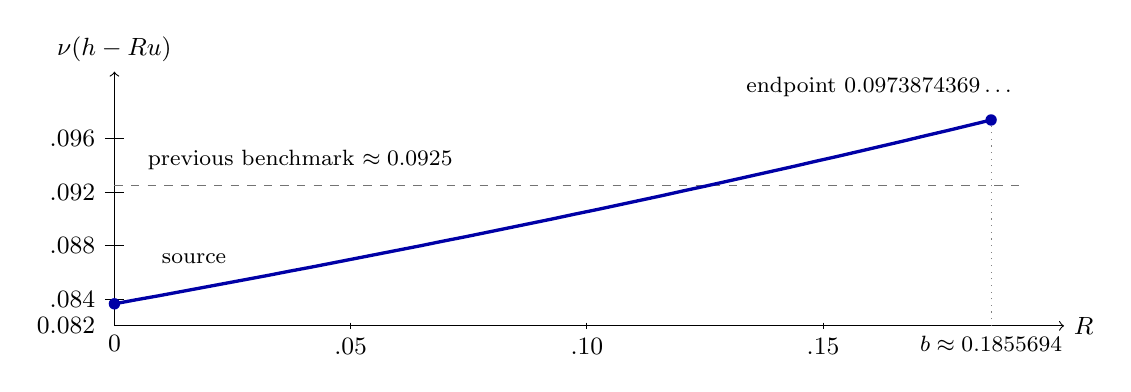
\begin{tikzpicture}[x=60cm,y=170cm,font=\small]
\draw[->] (0,0)--(.201,0) node[right] {$R$};
\draw[->] (0,0)--(0,.019) node[above] {$\nu(h-Ru)$};
\draw (.05,.00025)--(.05,-.00025) node[below] {$.05$};
\draw (.10,.00025)--(.10,-.00025) node[below] {$.10$};
\draw (.15,.00025)--(.15,-.00025) node[below] {$.15$};
\node[below] at (0,0) {$0$};
\node[left] at (-.002,0) {$0.082$};
\draw (-.002,0.002)--(.002,0.002);\node[left] at (-.002,0.002) {$.084$};
\draw (-.002,0.006)--(.002,0.006);\node[left] at (-.002,0.006) {$.088$};
\draw (-.002,0.010)--(.002,0.010);\node[left] at (-.002,0.010) {$.092$};
\draw (-.002,0.014)--(.002,0.014);\node[left] at (-.002,0.014) {$.096$};
\draw[black!55,dashed,line width=.45pt] (0,.0105)--(.193,.0105);
\node[anchor=south west,font=\footnotesize] at (.005,.0109) {previous benchmark $\approx0.0925$};
\draw[blue!65!black,very thick] plot coordinates {(0.000000000,0.001654706) (0.004639235,0.001950655) (0.009278470,0.002248707) (0.013917706,0.002548882) (0.018556941,0.002851204) (0.023196176,0.003155695) (0.027835411,0.003462380) (0.032474647,0.003771282) (0.037113882,0.004082425) (0.041753117,0.004395834) (0.046392352,0.004711533) (0.051031587,0.005029547) (0.055670823,0.005349903) (0.060310058,0.005672626) (0.064949293,0.005997743) (0.069588528,0.006325280) (0.074227764,0.006655264) (0.078866999,0.006987723) (0.083506234,0.007322685) (0.088145469,0.007660178) (0.092784704,0.008000231) (0.097423940,0.008342874) (0.102063175,0.008688135) (0.106702410,0.009036046) (0.111341645,0.009386636) (0.115980881,0.009739937) (0.120620116,0.010095980) (0.125259351,0.010454798) (0.129898586,0.010816422) (0.134537821,0.011180887) (0.139177057,0.011548225) (0.143816292,0.011918471) (0.148455527,0.012291659) (0.153094762,0.012667825) (0.157733998,0.013047004) (0.162373233,0.013429233) (0.167012468,0.013814548) (0.171651703,0.014202988) (0.176290939,0.014594590) (0.180930174,0.014989393) (0.185569409,0.015387437)};
\fill[blue!65!black] (0,0.001654706) circle[x radius=.0012,y radius=.00042];
\node[anchor=south west,font=\footnotesize] at (.008,.0039) {source};
\draw[gray,dotted] (0.185569409,0)--(0.185569409,0.015387437);
\fill[blue!65!black] (0.185569409,0.015387437) circle[x radius=.0012,y radius=.00042];
\node[anchor=south east,font=\footnotesize] at (.192,.0164) {endpoint $0.0973874369\ldots$};
\node[below,font=\footnotesize] at (0.185569409,0) {$b\approx0.1855694$};
\end{tikzpicture}

\caption{The achieved violation on the fixed path $h-Ru$, $0\le R\le b$.
The endpoint is the Shannon limit for this direction, proved achievable
in the almost-entropic cone. The vertical axis begins at $0.082$. The horizontal line is the rounded
previous benchmark. This is a plot of the construction, not a section of the unknown cone.}
\label{fig:path}
\end{figure}

\paragraph{Geometry along this path.}
The function $u$ contributes
$u(ABC)+u(ABD)-u(AB)-u(N)=1$ to $I(C;D\mid AB)$, so
\[
 I_{h-Ru}(C;D\mid AB)=b-R.
\]
The privacy bottleneck is therefore also the Shannon obstruction on this
path: every $R>b$ violates submodularity, while Theorem~\ref{thm:main}
realises every $0\le R\le b$. The nonnegative feasible rates on this
path are exactly $[0,b]$, both for $\AEcone$ and for $\Gamma_4$.
At the endpoint, $z(AB)=z(N)$ and every triple also has entropy $z(N)$,
placing $z/z(N)$ on these Shannon boundary hyperplanes.
Since $\Ing(h-Ru)=\Ing(h)<0$, its violation
$-\Ing(h)/(h(N)-3R)$ increases along the segment and is largest at $R=b$.
This proves optimality along this fixed source and direction.

Finally, since $z\in\AEcone$, finite entropic vectors approach $z$.
The score is continuous at $z$ because $z(N)>0$. Its upper bound in
\eqref{eq:scorebox} is strictly below $-0.09738$, proving the final
assertion of Theorem~\ref{thm:main}.
Exact finite realisability of $z$ remains open.
The next section gives an exact sampling procedure for
a suitable finite law, selected using the strict score margin.

\section{Generating a finite four-variable distribution}\label{sec:recipe}
The source table is already an explicit small distribution, but its
ordinary score is only about $-0.08365470562$. The score near
$-0.09738744$ belongs to the limiting vector $z$. We now describe actual
finite distributions which exceed the stated threshold, by selecting a conditional law.

Fix the strictly subcritical rational rate
\[
 R_0=\frac{371}{2000}=0.1855<b.
\]
The same exact entropy formulas certify
\[
 \frac{\Ing(h-R_0u)}{(h-R_0u)(N)}
 =-0.09738145760031\ldots<-0.09738.
\]
For all sufficiently large $n$, the matrix selected in the proof has a
conditional average profile with positive total entropy and score below
$-0.09738$. Let $h_w$ be the entropy vector of the four blocks given
$W=w$, and write $p_w=\Pr(W=w)$. Its average is
$\bar h=\sum_w p_w h_w$. The exact identity
\[
 \frac{\Ing(\bar h)}{\bar h(N)}
 =\sum_{w:h_w(N)>0}
    \frac{p_w h_w(N)}{\bar h(N)}
    \frac{\Ing(h_w)}{h_w(N)}
\]
shows that at least one positive-entropy fibre has score no larger than
the average. Fibres with $h_w(N)=0$ have all subset entropies and
$\Ing(h_w)$ equal to zero. This selects a fibre for the scalar score;
it does not make its fifteen coordinates equal to the average profile.

Once such $n$, $k=\lfloor nR_0\rfloor$, $M$ and $w$ have been chosen,
the following is an exact sampling recipe.
\begin{enumerate}[leftmargin=*]
\item Independently at each of $n$ positions, choose a column with
probabilities $(P,Q,T)$ and a uniform row among the eight table rows.
Read off $(X_{A,t},X_{B,t},X_{C,t},X_{D,t})$.
\item Compute $K_i=M(\chi(X_{i,1}),\ldots,\chi(X_{i,n}))^{\mathsf T}$
over $\F$, for $i=A,B,C$, and set $W=(K_A,K_B,K_C)$.
\item Retain the entire trial exactly when $W=w$; otherwise repeat it.
Output the four retained words, each in $\{0,1,2,3\}^n$.
\end{enumerate}
This rejection sampler terminates almost surely because $p_w>0$.
For four words $x=(x_A,x_B,x_C,x_D)$, if $\pi$ is the one-letter
rational table law, the output law is exactly
\[
 \Pr(X_A'=x_A,X_B'=x_B,X_C'=x_C,X_D'=x_D)
 =\frac{\mathbf1\{W(x)=w\}}{p_w}
      \prod_{t=1}^n\pi(x_{A,t},x_{B,t},x_{C,t},x_{D,t}).
\]
In particular all its probabilities are rational.

The proof guarantees suitable finite choices, but a practical block
length, matrix and fibre have not been computed. The strict rate
$R_0<b$ leaves a small privacy margin; no efficiency bound is claimed.



\section{Formal verification}\label{sec:verification}
Theorem~\ref{thm:main} has been formalised in Lean~4
(version~4.35.0-rc2), using Mathlib commit \texttt{065356127b1d}, and
checked by the Lean kernel. The declaration is
\texttt{ConditionalParityHashing.certified\_main} in
\texttt{CertifiedMain.lean}. In the notation of this paper it states:
\begin{enumerate}[label=(\roman*),leftmargin=*]
\item $h-Ru\in\AEcone$ for every $0\le R\le b$;
\item $z(N)>0$;
\item $-97387436923/10^{12}\le\Ing(z)/z(N)\le-97387436922/10^{12}$;
\item there exist an alphabet size $m$ and a law on $\{0,\ldots,m-1\}^4$
whose entropy vector $f$ has $f(N)>0$ and $\Ing(f)/f(N)<-0.09738$.
\end{enumerate}
The parameter in the final existential quantifier is an alphabet size,
rather than the block length used in the construction.

The definitions in this statement have their ordinary mathematical
meanings. \texttt{sourceLaw} is the rational law of Table~\ref{tab:source}.
\texttt{finiteEntropy} computes Shannon entropy in bits from the
finite-law marginals. \texttt{almostEntropicProfiles} is the topological
closure of those entropy vectors, in the space of functions on all
sixteen subsets of $N$, including the zero empty-set coordinate.
The checked semantic bridge identifies membership with simultaneous
$\varepsilon$-approximation of all coordinates by an actual finite law.
\texttt{paperJ} is precisely~\eqref{eq:J}; \texttt{criticalRate} is
$h(N)-h(AB)$, proved equal to $I(C;D\mid AB)$; \texttt{shiftedProfile}~$R$
is $h-Ru$; and \texttt{candidate} is $z$.
The general six-test criterion is also checked, through the ten-threshold
argument and its six-to-ten reduction. The axiom report uses only
\texttt{propext}, \texttt{Classical.choice} and \texttt{Quot.sound}.

The formal proof uses the same bounded-deficit hashing argument as
Appendix~\ref{app:hash}. Its source-threshold comparisons and score
bounds use certified $20$-term artanh-series enclosures, while the written
threshold comparisons are analytic and the independent Python checker
uses the rational series in Appendix~\ref{app:numerical}.
The finite-alphabet clause follows formally by density and continuity;
the explicit fibre selection and sampling description of
Section~\ref{sec:recipe}, and the path-optimality discussion, are not
separately formalised. The proof package contains the pinned Lean sources (27 proof modules and
one verification file), a fresh-directory rebuild script with the axiom
report it produced, and two exact rational checkers written for the
Python standard library. The paper, manuscript sources, Lean proof and
verification evidence are available in the
\href{https://github.com/SR123/conditional-parity-hashing}{GitHub repository}.
The archived version is identified by
\href{https://doi.org/10.5281/zenodo.23662511}{doi:10.5281/zenodo.23662511}.
The paper and its sources are licensed under CC BY 4.0; code is
licensed under Apache-2.0.

\section{Discussion}
The construction gives an inner bound for the full almost-entropic cone.
The maximum Ingleton violation, extremality of $z$, and exact finite
realisability of $z$ remain open. The six-test criterion suggests looking
for other finite sources with local algebraic relations that permit
larger structured subtractions. Extending the construction to other
matroidal information profiles may provide further inner bounds.


\appendix
\section{Proof of the simultaneous hashing lemma}\label{app:hash}
\begin{proof}
Fix one pair $(Z,G)$ in the finite list, put $H=H(Z\mid G)$ and
$\varepsilon=(H-R)/2>0$, and take $n\ge1$.
For a positive-probability value $g$ of $G^n$, write
$p(z\mid g)=\Pr(Z^n=z\mid G^n=g)$. Call $(z,g)$ typical when
$p(z\mid g)\le2^{-n(H-\varepsilon)}$, and let $a_n$ be the probability
of the typical event. All logarithms in this proof are to base two.

For a fixed binary matrix $M$ define
\[
 q_M(z,g)=\Pr(MZ^n=Mz\mid G^n=g).
\]
Thus $H(MZ^n\mid G^n)=\E[-\log q_M(Z^n,G^n)]$ is a sum of nonnegative
terms. Drop the atypical terms and average over a uniform random matrix
$M$, independently of the source. If $a_n>0$, Jensen's inequality gives
\[
 \E_M H(MZ^n\mid G^n)
 \ge-a_n\log\E\bigl[\E_M q_M(Z^n,G^n)\mid\text{typical}\bigr].
\]
Two distinct binary strings collide under a uniform $k\times n$ matrix
with probability $2^{-k}$: each row has a uniform dot product with their
nonzero difference, and the rows are independent. Consequently
\[
 \E_M q_M(z,g)
 =\sum_{z'}p(z'\mid g)\Pr_M(Mz'=Mz)
 \le p(z\mid g)+2^{-k}.
\]
On typical pairs the right-hand side is at most
$2^{-k}(1+2^{k-n(H-\varepsilon)})$. Write $x=2^{k-n(H-\varepsilon)}$. Since $\log_2(1+x)\le x/\ln2$
and $a_n\le1$, the preceding estimate gives
\[
 \E_M H(MZ^n\mid G^n)
 \ge a_n\bigl(k-\log_2(1+x)\bigr)
 \ge a_nk-\frac{x}{\ln2}.
\]
Subtracting from $k$ and using $k\le nR=n(H-2\varepsilon)$ gives
\begin{equation}\label{eq:hashbound}
 \E_M\,[k-H(MZ^n\mid G^n)]
 \le (1-a_n)k+\frac{2^{k-n(H-\varepsilon)}}{\ln2}
 \le (1-a_n)nR+\frac{2^{-n\varepsilon}}{\ln2}.
\end{equation}
If $a_n=0$, the first bound holds directly from nonnegativity of entropy,
so no conditioning on a null event is required.

On the finite positive support, $\iota=-\log p(Z\mid G)$ is bounded,
with mean $H$ and a finite variance $v$. For the $t$th copy put $\iota_t=-\log p(Z_t\mid G_t)$. Independence gives
$-\log p(Z^n\mid G^n)=\sum_{t=1}^n\iota_t$. Chebyshev's inequality
therefore yields $1-a_n\le v/(n\varepsilon^2)$. It follows that
\[
 \E_M\,[k-H(MZ^n\mid G^n)]\le\frac{vR}{\varepsilon^2}+\frac1{\ln2}.
\]
Sum this bound over the finite list. Its sum is a constant independent of
$n$, and some deterministic matrix has a deficit sum no larger than the
average. For $n=0$ every key is empty and every deficit is zero.
\end{proof}

\section{Exact numerical enclosure}\label{app:numerical}
The following rational computation certifies~\eqref{eq:scorebox}; it does
not enter the membership proof. For a rational $x\in[1,2]$ put
$y=(x-1)/(x+1)$ and
\begin{equation}\label{eq:series}
 \ell_m(x)=2\sum_{j=0}^{m-1}\frac{y^{2j+1}}{2j+1},\qquad
 0\le\ln x-\ell_m(x)\le
 \frac{2y^{2m+1}}{(2m+1)(1-y^2)}.
\end{equation}
This is the positive series for $2\operatorname{arctanh}y$, with its tail
bounded geometrically. For each positive rational argument $w$, write
$w=2^\ell x$, $1\le x<2$, and enclose
$\log_2w=\ell+\ln x/\ln2$ using~\eqref{eq:series} with $m=42$ for $x$
and $2$. Rational interval arithmetic in~\eqref{eq:b},
\eqref{eq:Jformula} and~\eqref{eq:den} gives~\eqref{eq:scorebox}.
The accompanying \texttt{verify\_paper.py} implements exactly this recipe
using only rational arithmetic from the Python standard library and also
checks the finite source identities. The displayed decimal bounds are
outward rounded; the exact entropy expressions define the point.

The Lean proof independently encloses the same logarithms with Mathlib's $20$-term artanh-series bounds. Both calculations are rigorous.

\section*{Acknowledgements and contributions}
S\o ren Riis is the creator and coordinator of the project, responsible
for its research direction and outline. Mathematical development,
computation and verification were carried out with Astra/Codex and
Claude; Claude also contributed the Lean formalisation and adversarial
review, and Astra/Codex checked the formal statements and rebuilt the
proof package. These AI-assisted checks do not constitute independent
human peer review.

The source family is due to Mat\'u\v{s} and Csirmaz; the compression,
privacy-amplification and conditioning methods build on the works cited
above. The work of Dougherty, Freiling, Zeger and Yeung supplies much of
the surrounding information-inequality framework~\cite{DFZ,ZY,ZY98}.
These attributions do not imply endorsement by the researchers named.


\begin{thebibliography}{99}\footnotesize\raggedright\setlength{\itemsep}{0pt}
\bibitem{DFZ}
R. Dougherty, C. Freiling and K. Zeger,
``Non-Shannon information inequalities in four random variables,''
arXiv:1104.3602, 2011.
\href{https://arxiv.org/abs/1104.3602}{arXiv:1104.3602}.

\bibitem{MC}
F. Mat\'u\v{s} and L. Csirmaz, ``Entropy region and convolution,''
\emph{IEEE Trans. Inf. Theory}, vol.~62, no.~11, pp.~6007--6018, 2016.
\href{https://doi.org/10.1109/TIT.2016.2601598}{doi:10.1109/TIT.2016.2601598};
\href{https://arxiv.org/abs/1310.5957v1}{arXiv:1310.5957v1} (2013).

\bibitem{ZY}
Z. Zhang and R. W. Yeung,
``A non-Shannon-type conditional inequality of information quantities,''
\emph{IEEE Trans. Inf. Theory}, vol.~43, no.~6, pp.~1982--1986, 1997.
\href{https://doi.org/10.1109/18.641561}{doi:10.1109/18.641561}.

\bibitem{MS95}
F. Mat\'u\v{s} and M. Studen\'y, ``Conditional independences among four random
variables I,'' \emph{Combin. Probab. Comput.}, vol. 4,
no. 3, pp. 269--278, 1995.
\href{https://doi.org/10.1017/S0963548300001644}{doi:10.1017/S0963548300001644}.

\bibitem{HRSV00}
D. Hammer, A. Romashchenko, A. Shen and N. Vereshchagin,
``Inequalities for Shannon entropy and Kolmogorov complexity,''
\emph{J. Comput. Syst. Sci.}, vol. 60, no. 2,
pp. 442--464, 2000.
\href{https://doi.org/10.1006/jcss.1999.1677}{doi:10.1006/jcss.1999.1677}.

\bibitem{ZY98}
Z. Zhang and R. W. Yeung,
``On characterization of entropy function via information inequalities,''
\emph{IEEE Trans. Inf. Theory}, vol.~44, no.~4, pp.~1440--1452, 1998.
\href{https://doi.org/10.1109/18.681320}{doi:10.1109/18.681320}.

\bibitem{MatusInfinite}
F. Mat\'u\v{s}, ``Infinitely many information inequalities,''
in \emph{Proc. IEEE Int. Symp. Inf. Theory}, 2007, pp.~41--44.
\href{https://doi.org/10.1109/ISIT.2007.4557201}{doi:10.1109/ISIT.2007.4557201}.

\bibitem{KR}
T. Kaced and A. Romashchenko,
``Conditional information inequalities for entropic and almost entropic points,''
\emph{IEEE Trans. Inf. Theory}, vol.~59, no.~11, pp.~7149--7167, 2013.
\href{https://doi.org/10.1109/TIT.2013.2274614}{doi:10.1109/TIT.2013.2274614};
\href{https://arxiv.org/abs/1207.5742}{arXiv:1207.5742}.

\bibitem{Ingleton71}
A. W. Ingleton, ``Representation of matroids,'' in
\emph{Combinatorial Mathematics and its Applications}, D. J. A. Welsh, Ed.
London, UK: Academic Press, 1971, pp. 149--167.

\bibitem{Chang}
J. Chang, ``Improved bounds on the Ingleton score of four random variables,''
arXiv:2610.05168, Oct.~4, 2026.
\href{https://arxiv.org/abs/2610.05168}{arXiv:2610.05168}.

\bibitem{BN}
N. Boston and T.-T. Nan,
``Violations of the Ingleton inequality and revising the four-atom conjecture,''
\emph{Kybernetika}, vol.~56, no.~5, pp.~916--933, 2020.
\href{https://doi.org/10.14736/kyb-2020-5-0916}{doi:10.14736/kyb-2020-5-0916}.

\bibitem{CNN}
S. Zhang, N. Liu, W. Kang and H. Permuter,
``Optimizing distributions for associated entropic vectors via generative convolutional neural networks,''
\emph{Entropy}, vol.~26, no.~8, Art. no.~711, 2024.
\href{https://doi.org/10.3390/e26080711}{doi:10.3390/e26080711}.

\bibitem{Matus}
F. Mat\'u\v{s}, ``Two constructions on limits of entropy functions,''
\emph{IEEE Trans. Inf. Theory}, vol.~53, no.~1, pp.~320--330, 2007.
\href{https://doi.org/10.1109/TIT.2006.887090}{doi:10.1109/TIT.2006.887090}.

\bibitem{BBCM}
C. H. Bennett, G. Brassard, C. Cr\'epeau and U. M. Maurer,
``Generalized privacy amplification,''
\emph{IEEE Trans. Inf. Theory}, vol.~41, no.~6, pp.~1915--1923, 1995.
\href{https://crypto.cs.mcgill.ca/~crepeau/PDF/ASPUBLISHED/BBCM95.pdf}{Author-hosted journal copy}.

\bibitem{Csiszar96}
I. Csisz\'ar, ``Almost independence and secrecy capacity,''
\emph{Problems Inf. Transm.}, vol.~32, no.~1, pp.~40--47, 1996.
\url{https://www.mathnet.ru/eng/ppi319}.

\bibitem{RW}
R. Renner and S. Wolf,
``Simple and tight bounds for information reconciliation and privacy amplification,''
in \emph{Advances in Cryptology---ASIACRYPT 2005}, ser. Lecture Notes in Computer Science, vol.~3788. Springer, 2005, pp.~199--216.
\url{https://crypto.ethz.ch/publications/RenWol05.html}.
\end{thebibliography}
\end{document}
